%------------------------------------------------- Modélisation -------------------------------------------------%
	
	\part{Modélisation}
	\parttoc
	
	\setcounter{chapter}{0} % Pour recommencer la numérotation des chapitres à 1
	\setcounter{section}{0} % Pour recommencer la numérotation des section à 1
	
	\renewcommand*{\theHchapter}{\thepart.\thechapter}
	\chapter{Introduction}
	La phase de conception est la phase permettant de mettre en place les différentes étapes nécessaires à la réalisation de notre projet. Elle inclue des schémas et des diagrammes structurés représentant les étapes et les fonctionnalités de notre future application. La phase de conception est la dernière étape avant la programmation logicielle, elle doit donc être précise et fiable, dans le but de minimiser au maximum les risques d'erreurs d'implémentation. 
	
	La phase de conception s'appuie en grande partie sur ce qui a été mis en place dans le cahier des charges de la phase 1. Les différentes réunions avec les différents protagonistes du projet ont permis de fixer les objectifs prioritaires à concevoir en priorité. Dans notre projet, il s'agira donc de trouver un moyen efficace de transcrire la voix en texte, et de pouvoir exploiter cette transcription. Pour  cela, il sera nécessaire d'établir des connexions entre notre module et le serveur de la plate-forme Project2Cloud. Nous nous sommes pour cela initié au techniques de transcription vocale ( Speech-to-text ) au travers de modules libres existant.

	 Dans ce compte rendu de phase de conception, nous présenterons le module développé sous différents aspects (diagrammes, partons de conception). Nous estimerons également la charge de travail prévue, via la méthode COCOMO. Cet méthode nous donnera des indications sur le volume de travail à fournir en fonction des choix techniques effectués avec les tuteurs enseignants et entreprise. 


	\chapter{Principe général}
	Notre module sera développé à part, et ne sera pas directement intégré dans la plate-forme P2C. Il devra cependant échanger des informations contenu sur le serveur de la plate-forme. Les vidéos enregistrées sur le serveur devront être traité par notre module, qui en proposera une transcription de type Speech-to-text. La transcription ainsi effectuée sera renvoyée au serveur. Idéalement, un système d'échange module-serveur pourrait être mis en place, permettant un dialogue continu entre les deux instances. Ceci permettrait de rendre le module auto-didacte et d'améliorer significativement la qualité de la transcription proposée.
	
	\begin{figure}[H]
		\begin{center}
			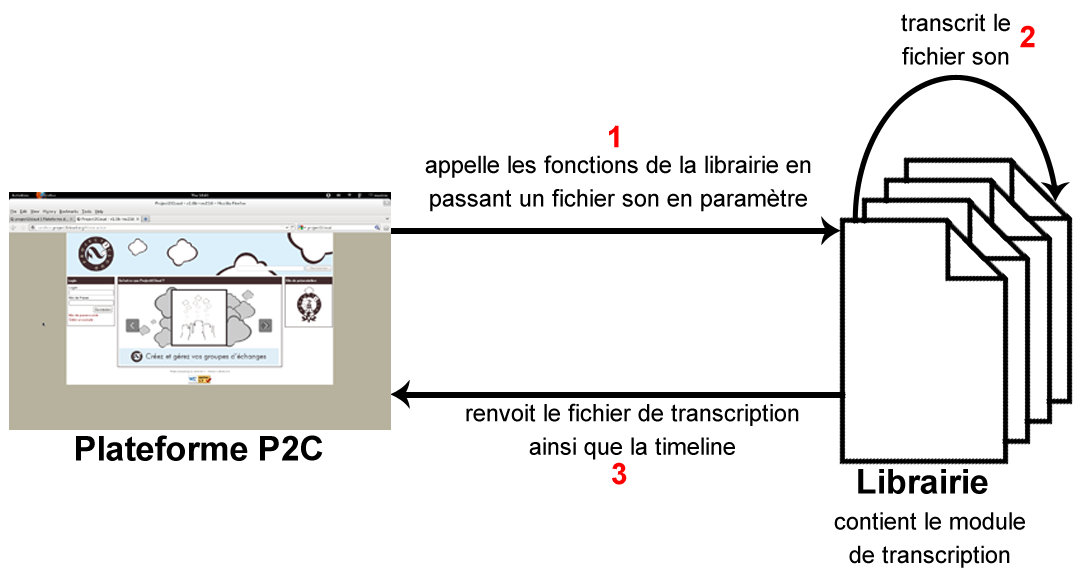
\includegraphics[width=12cm]{shema_general_modelisation}
			\caption{Shéma du principe général}
			\label{sequence_transcription}
		\end{center}
	\end{figure}

	
	
	
	\chapter{Transcription}
	Le module va périodiquement interroger la base de donnée pour détecter les nouveaux fichiers son encodés disponibles. Lorsque tel est le cas, il lancera ce fichier pour le transcrire grâce à son modèle de reconnaissance. De plus, à chaque mot clé reconnu (mot clé entré pas l'utilisateur), il l'indexera dans un fichier XML. Dans ce dernier, seront associés un mot clés et une donnée temporelle, correspondant au moment où ce mot clé a été prononcé dans la vidéo.

	A chaque fichier de transcription sera associé un numéro de version. Ainsi, lorsque le modèle de reconnaissance a suffisamment évolué, une nouvelle transcription sera faite.
	
	\begin{figure}[H]
		\begin{center}
			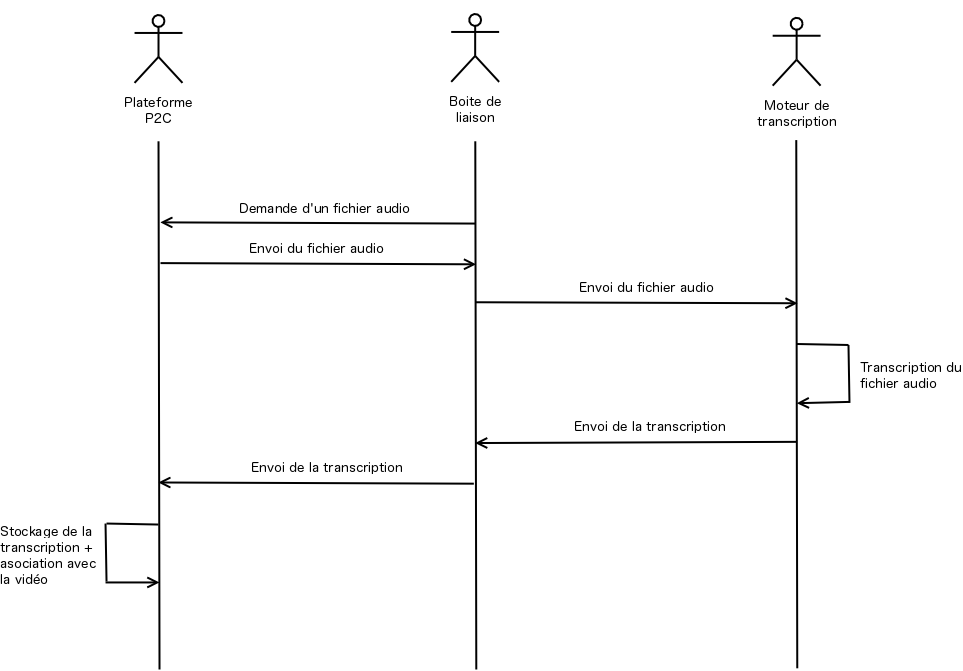
\includegraphics[width=12cm]{sequence_transcription}
			\caption{Diagramme de séquence entre la plateforme et le module de transcription}
			\label{sequence_transcription}
		\end{center}
	\end{figure}

	
	\section{Module de transcription}
	Pour la reconnaissance automatique de la parole, nous avons choisi d'utiliser l'application Sphinx 4\footnote{L'application est disponible à l'adresse suivante : http://cmusphinx.sourceforge.net/sphinx4/}. Son architecture est modélisée dans la figure \ref{architecture_sphinx_4} :
	
	\begin{figure}[H]
		\begin{center}
			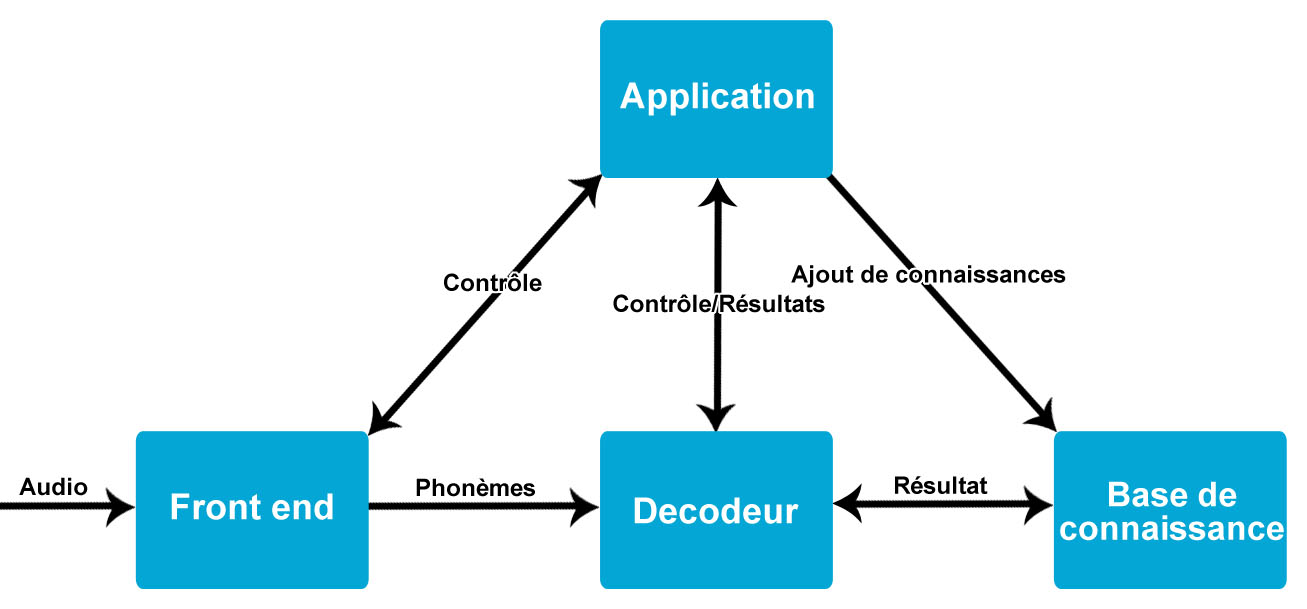
\includegraphics[width=12cm]{architecture_sphinx_4}
			\caption{Architecture du logiciel Sphinx 4}
			\label{architecture_sphinx_4}
		\end{center}
	\end{figure}

\begin{description}
	\item{\textbf{Front end}} : le front end découpe la voix enregistrée en différentes parties et les prépare pour le décodeur.
	\item{\textbf{Base de connaissance}} : la base de connaissance est l’information qu’utilise le décodeur pour déterminer les mots et les phrases prononcés. La base de connaissance est composée :
	
	\begin{itemize}
		\item d’un dictionnaire
		\item classification des mots
		\item prononciation des mots (un mot peut avoir plusieurs prononciations)
		\item prononciation représentée comme des sons ou dans d’autres unités
		\item d’un modèles acoustique
		\item d’un modèle de langage
	\end{itemize}
	De plus, une base de connaissance :
	\begin{itemize}
		\item peu varier en taille, de quelque mots à plusieurs centaines de milliers
		\item décrit ce qui peut être dit dans un contexte bien spécial
		\item aide à rétrécir l’espace de recherche
	\end{itemize}
		
Il y a trois sortes de modèle de langage : le plus simple est utilisé pour les mots isolés, le deuxième pour les applications basées sur des commandes et des contrôles et le dernier pour le langage courant.
	
	\item{\textbf{Décodeur}} : le décodeur est le coeur de Sphinx 4. C’est lui qui traite les informations reçues depuis le Front end, les analyse et les compare avec la base de connaissance pour donner un résultat à l’application
	
	
	
\end{description}

	
	\chapter{Amélioration de modèle}
	
	
	\chapter{test}
	Notre application est composée de deux tests  :  transcription et mappage temporelle de la transcription

	\section{tests unitaires}

	\subsection{tests boite noire}
	
	
	
	
	
	
